\chapter[Sistema Adaptativo de Vídeos Interativos]{Sistema Adaptativo de Vídeos Interativos}

Tendo como base as teorias apresentadas, foi desenvolvido um sistema que utiliza o modelo arquitetural MVC e que contempla duas funcionalidades principais: um módulo para autoria de cursos compostos por vídeos interativos e um módulo para visualização adaptativa destes cursos, que contemple adaptações de conteúdo e navegação. 

Para facilitar a compreensão do trabalho técnico desenvolvido, este capítulo foi subdividido em cinco tópicos: modelagem do domínio, arquitetura do software, gerência de configuração, testes e aspectos gerais. 

\section{Modelagem do Domínio}

O modelo do domínio do software pretende apresentar os elementos que compõem a lógica do sistema e como eles foram organizados para que os objetivos do trabalho pudessem ser alcançados. É importante ressaltar que estes modelos apresentados foram evoluídos no decorrer do desenvolvimento até alcançarem um nível estável, já que o método seguido foi interativo e incremental segundo as práticas do \textit{Scrum}.

\begin{figure}[h!]
	\centering
  	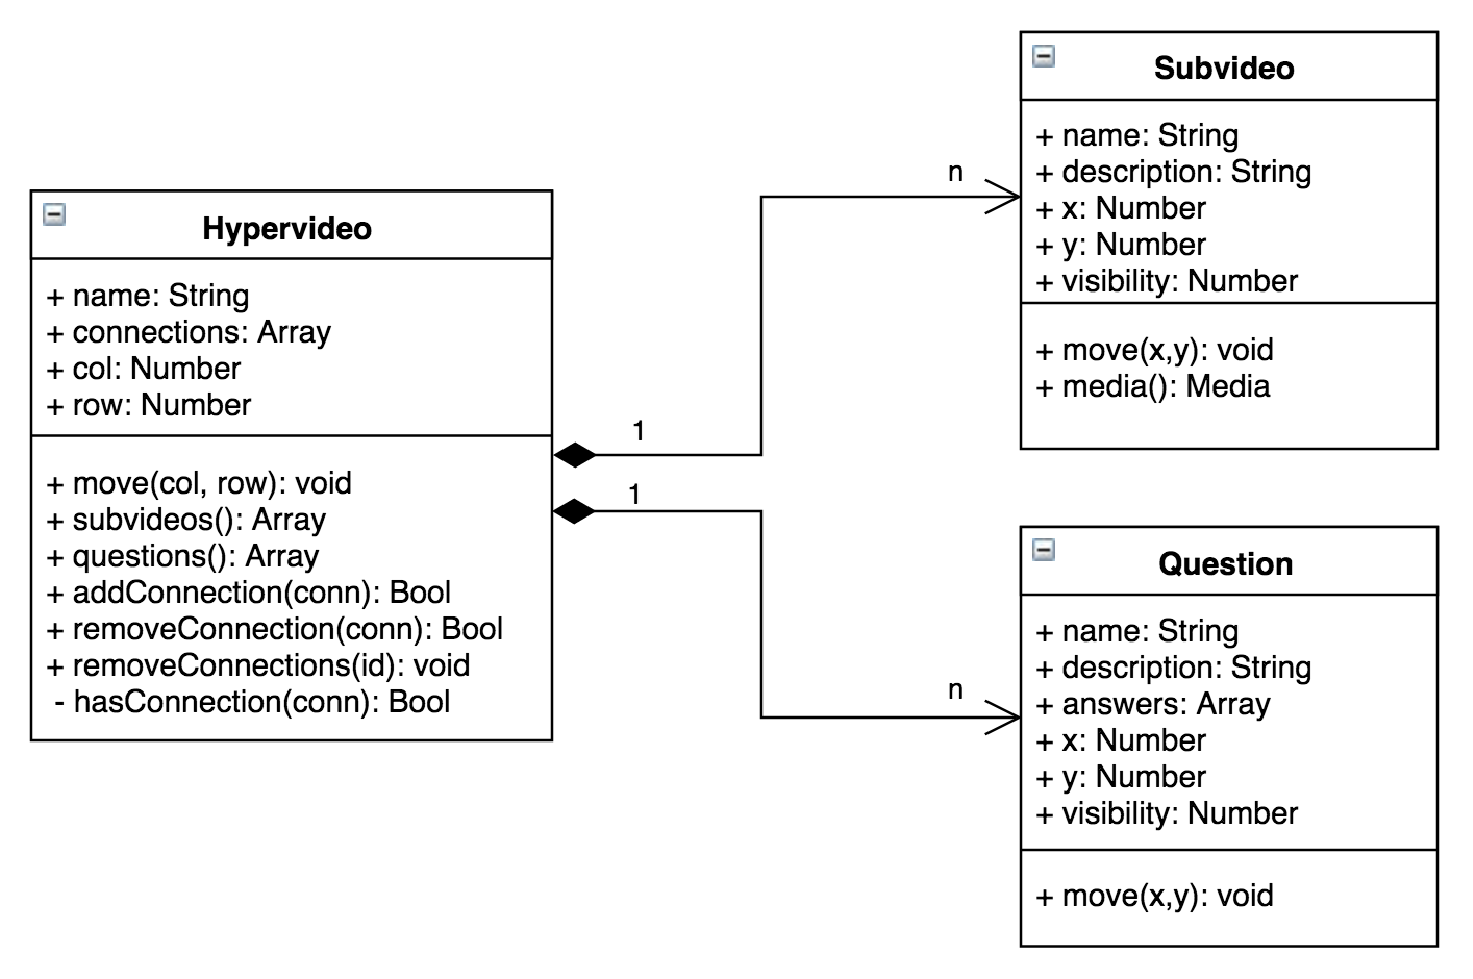
\includegraphics[width=.6\linewidth]{figuras/video.eps}
  	\caption{Diagrama do vídeo interativo proposto}
  	\label{fig:video}
\end{figure}

Primeiramente, foi modelado um vídeo interativo que pudesse ser utilizado na construção de um curso. Levando em consideração os princípios do design multimídia, os vídeos interativos possuem pouco espaço para textos escritos na tela; são formados por subvídeos interligados segundo definido pelo professor autor; possuem questões a serem respondidas ao longo da apresentação do vídeo e devem ser adaptativos segundo os diferentes perfis de usuário. Além disso, um vídeo interativo deve possuir as informações necessárias para que ocorra a quantização da rede, ou seja, para cada usuário que o acesse, deve existir uma avaliação e uma confiabilidade atribuidos a ele, bem como uma posição em um plano bidimensional referente ao mapa conceitual do curso ao qual o vídeo interativo pertence. 

\begin{figure}[h!]
	\centering
  	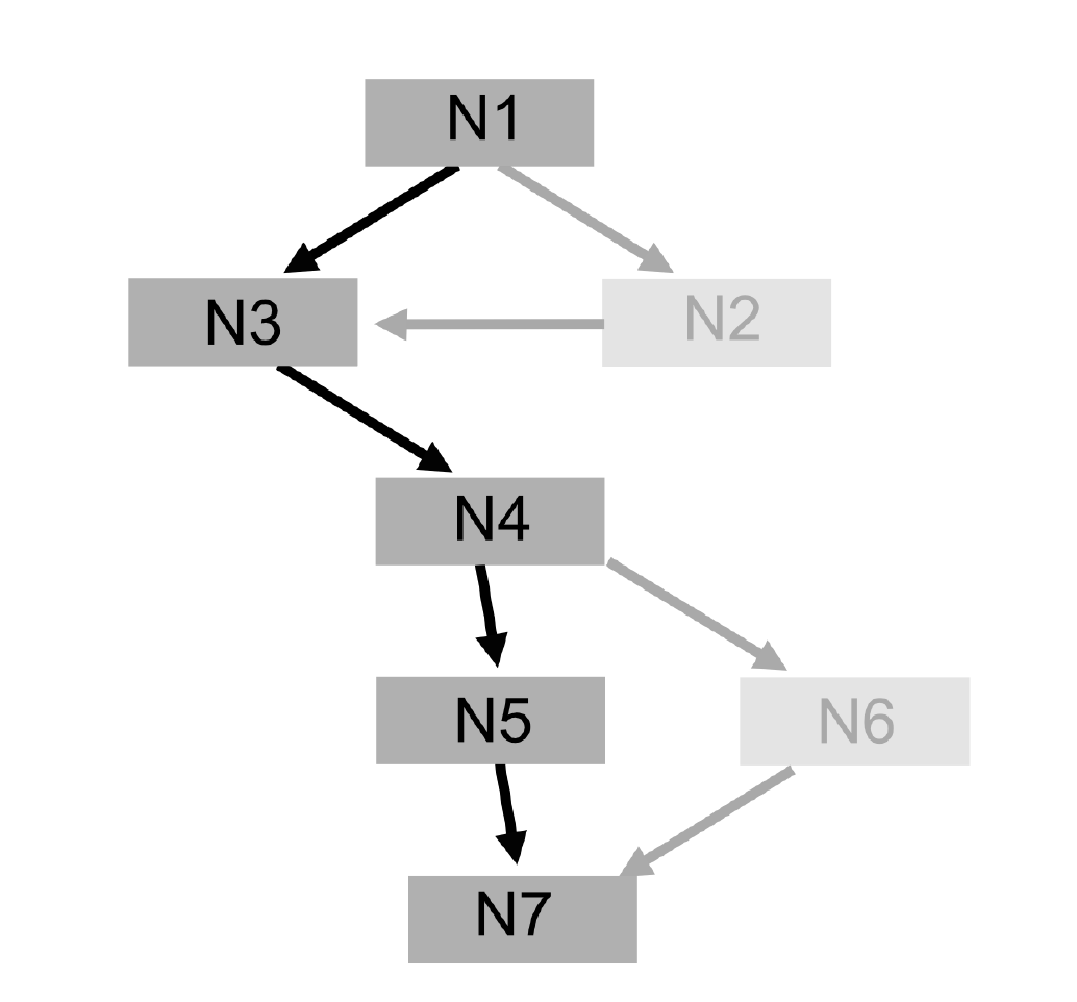
\includegraphics[width=.3\linewidth]{figuras/estrutura.eps}
  	\caption{Adaptação do hypervideo por meio da ocultação dos nodos N2 e N6}
  	\label{fig:estrutura}
\end{figure}

Cada subvídeo possui informações básicas sobre a mídia de vídeo que será apresentada por ele, como título e uma breve descrição do conteúdo. Além disso, possuem um nível de visibilidade para serem apresentados apenas ao perfil específico para o qual foi projetado, garantindo assim a capacidade de adaptação a nível de conteúdo. A fig. \ref{fig:video} apresenta um diagrama do vídeo interativo que no sistema é denominado Hypervideo.

Por meio da figura \ref{fig:video}, é possível perceber que existe uma lista de conexões para cada Hypervideo, essa lista representa o conjunto de arestas do grafo que tem como vértices os subvídeos e questões pertencentes a o vídeo interativo. Como visto no capítulo anterior, as teorias behavioristas apresentam o conteúdo de forma sequencial e linear, já as linhas cognitivistas compreendem estruturas de decisão e caminhos distintos para cada aprendiz. A figura \ref{fig:estrutura} mostra como essa estrutura de grafo pode se adaptar para adequar-se a ambas as formas de apresentação.

\begin{figure}[h!]
	\centering
  	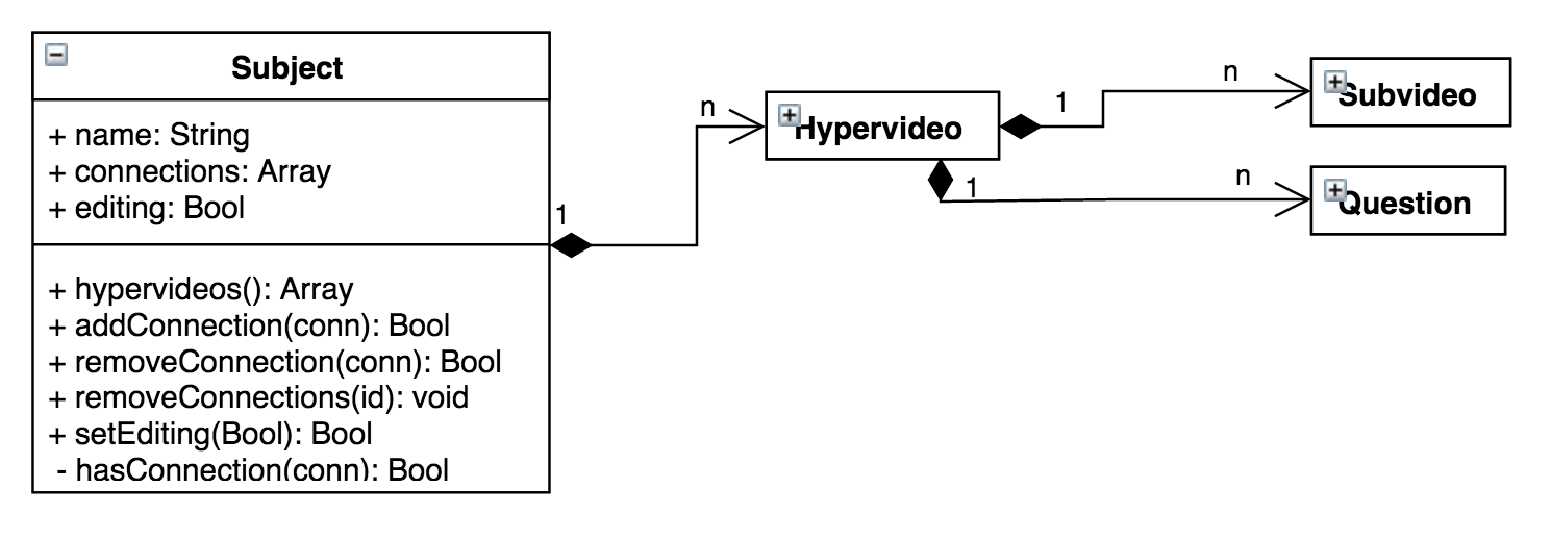
\includegraphics[width=.7\linewidth]{figuras/curso.eps}
  	\caption{Diagrama da estrutura do curso proposto}
  	\label{fig:curso}
\end{figure}

Para que fosse possível desenvolver uma adaptação da navegação que utilizasse a QRN, foi necessário modelar também a estrutura do curso que comportasse os hypervídeos e as informaçõs necessárias para os cálculos. Dessa forma, é proposto que um curso possua também, uma estrutura de grafo que tenha como vértices os seus Hypervideos, e que as conexões criadas pelo professor representem as ligações conceituais entre os tópicos apresentados em cada hypervídeo. A figura \ref{fig:curso} apresenta o modelo relativo ao curso que foi denominado \textit{Subject}.

A próxima modelagem feita foi referente aos dados do usuário: cursos que assiste, cursos construídos por ele, percentual de conclusão de um curso, questões respondidas, hypervideos assistidos, etc. Todas essas informações requereram modelos que vinculassem cada elemento de um curso ao usuário para que se pudesse calcular os coeficientes de quantização para os nodos da rede. A figura \ref{fig:userdata} mostra o modelo de domínio completo do \textit{software}.

\begin{figure}[h!]
	\centering
  	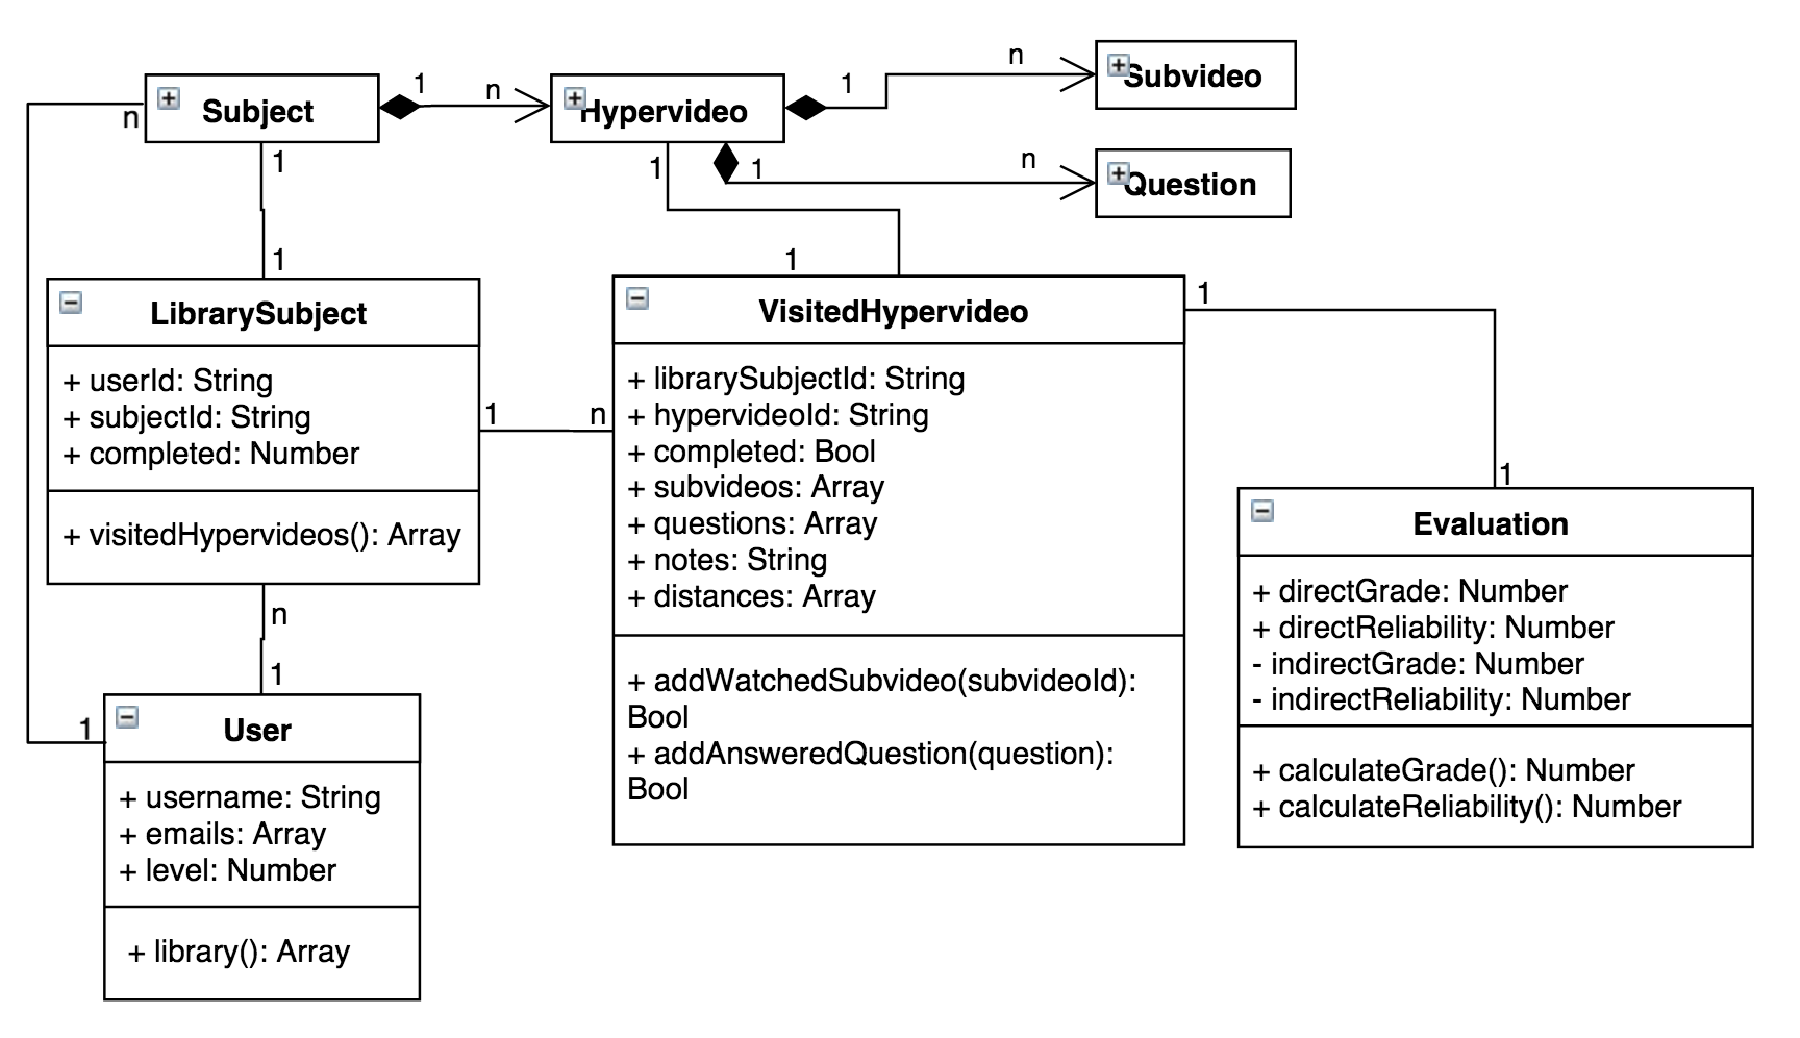
\includegraphics[width=.8\linewidth]{figuras/userdata.eps}
  	\caption{Diagrama sobre informações referentes a relação usuário \(\times\) curso}
  	\label{fig:userdata}
\end{figure}
